
\section{Stokes Parameters}
\label{sec:stokes}

It is important to describe polarisation, as it clarifies key considerations in the receiver design. \citet{tinbergen_1996} provides a good reference on the use of polarimetry in astronomy and was used extensively in the following summary. Detailed descriptions have been avoided.

An electromagnetic wave propagates in a transverse fashion and exhibits vector characteristics. At any instant, the vector describing the electric field can be resolved into two components at right angles to each other. For unpolarised radiation there is no lasting relationship between these two components. For polarised radiation, however, an amplitude and phase relationship does exist, such that the vector comprised of the two components traces out an ellipse, circle or straight line. These three states give rise to the terms \textit{elliptical, circular and linear} polarisation respectively.  

The Stokes parameters (I,Q,U and V) fully describe the state of polarisation. The parameter I characterises the intensity of the incoming radiation, Q and U characterise the state of linear polarisation and V the state of circular polarisation. Measuring I, Q, U and V at radio frequencies can be done by correlating orthogonal modes of the incoming radiation. 

\citeasnoun{tinbergen_1996} also points out the significant relationship, that left (L) and right (R) hand \textit{circular polarisation} the Stokes parameters are related to the correlations by 

\begin{eqnarray}
& I &= LL^{*} + RR^{*}  \label{eq:stokes_circ_I} \\
& Q &= 2Re(LR^{*}) \label{eq:stokes_circ_Q}\\
& U &= -2Im(LR^{*}) \label{eq:stokes_circ_U}\\
& V &= LL^{*}-RR^{*} \label{eq:stokes_circ_V}
\label{eq:stokes_circ}
\end{eqnarray} 

(where $LL^{*}$ denotes the auto-correlation of the left circular polarisation for example) while for X and Y \textit{linear polarisations} the parameters relate to the correlations by


\begin{eqnarray}
& I &= XX^{*} + RR^{*} \label{eq:stokes_lin_I} \\ 
& Q &= XX^{*} - YY^{*} \label{eq:stokes_lin_Q}\\
& U &= 2Re(XY^{*}) \label{eq:stokes_lin_U}\\
& V &= 2Im(XY^{*}) \label{eq:stokes_lin_V}
\label{eq:stokes_lin}
\end{eqnarray} 

The significance of the equations is apparent when we consider the type of polarisation we are trying to measure. Since Q, U and V will be small percentages, it is preferable to use a form that produces measurements using correlation rather than the less sensitive differencing operation. We can see from the equations that equipment designed for measuring \textit{linear polarisation} (i.e Q and U) should use correlations of circular polarisation (as shown by Equation~\ref{eq:stokes_circ_Q} and Equation~\ref{eq:stokes_circ_U}), while equipment designed for measuring \textit{circular polarisation} (i.e V) should use correlations of linear polarisation (see Equation~\ref{eq:stokes_lin_V}). 


For C-BASS we are interested in Galactic polarised emissions. This will be dominated by the synchrotron radiation mechanism \cite{Reich:2006iq},\cite{Bennett2003} producing linear polarisation, hence we choose to use correlations of circular polarisation.


\section{Pseudo-correlation architecture}
\label{sec:pseudoCorrelation}
The polarimeter will be built using a pseudo-correlation architecture (see \fign{fig:pseudo_correlation} and \fign{fig:digital_receiver_mine}). This is a differential receiver architecture (with continuous comparisons between the sky temperature and a stable reference load, see \fign{fig:pseudo_correlation}) with the associated benefits of improved stability with amplifier gain fluctuations.  \citeasnoun{Mennella2003b} and \citeasnoun{Seiffert2002} describe this receiver architecture as implemented on the Planck-LFI instrument, and note the improvement over a a Dicke switched scheme (i.e switching between load and sky) by avoiding the need for an active switch in the receiver chain and improving the sensitivity by $\sqrt{2}$. 

We are currently using an analogue pseudo-correlation polarimeter for the OVRO antenna. The receiver consists of a front end cooled to 4~K. The cooled section comprises a ortho-mode transducer (OMT) which separates the incoming signal (defined hereafter as $T_{sky}$) into orthogonal linear polarisations, which are then converted to circular polarisation using 90\degt hybrids. The reason for the conversion to circular polarisation is described in Appendix~\ref{sec:stokes}. Each of the orthogonal circular polarisations (left (LHC) and right (RHC) hand circular polarisation) is then coupled to a reference load signal ($T_{ref}=4K$) through a 180$^{\circ}$ hybrid producing two signals ($T_{1}=T_{sky}+T_{ref}$ and $T_{2}=T_{sky}-T_{ref}$) which propagate through independent signal paths. In the first signal path, the signal passes through a phase switch applying a delay that alternates between 0 and 180\degt, while the other signal path is routed through a similar phase switch (for symmetry) with no change in phase being applied. The signals are then recombined (using a 180\degt hybrid in the Planck architecture) producing the output sequence in \fign{fig:pseudo_correlation}. The signals are then appropriately correlated to measure the Stokes parameters as described in \secn{sec:stokes}. In the new digital receiver the signals will be recombined in the frequency domain, after taking fast-Fourier transforms (FFT) of each of the signals independently. The correlations will then be implemented digitally.

This continuous comparison (again, see \fign{fig:pseudo_correlation}) between the sky and reference load temperatures is useful for removing gain fluctuations in the amplifiers, since fluctuations will effect both  $T_{sky}$ and the known $T_{ref}$ equally. In addition, the fast switching reduces the impact of 1/f (or pink) noise in the amplifiers \cite{Seiffert2002}). 



\section{Digital Implementation}
\label{sec:digitalImplementation}
The new digital receiver will perform a similar operation to the analogue receiver and will be implemented on a CASPER \textit{ROACH} board\footnote{http://casper.berkeley.edu/}. Two 500~MHz bands will be captured using 1~Gsps analogue-to-digital converters (ADC), after suitable heterodyning of the 4.5~GHz$\rightarrow$5.5~GHz frequency band into the 0$\rightarrow$1000~MHz band. The two 500~MHz bands are defined by a 0$\rightarrow$500~MHz low pass filter (first Nyquist zone) and a 500MHz$\rightarrow$1000~MHz band pass filter (second Nyquist zone) as depicted in the diagram in \fign{fig:digital_receiver} and \fign{fig:digital_receiver_mine}. A n=128 fast fourier transform (FFT) is performed by the \textit{Virtex-5} field-programmable gate array (FPGA) providing 64 channels ( i.e the real components of the n=128 FFT)  and a bin width  of 7.8~MHz per channel across each 500~MHz band. Increasing the spectral resolution further would only be possible on a larger FPGA.

\subsection{Advantages of the Digital Implementation}
The analog polarimeter is designed with a single 1~GHz band, with correlations performed using analog components (90  $^{\circ}$ and 180 $^{\circ}$ hybrids). A similar approach could be used in a digital receiver. The incoming data is sampled, and the analog components emulated with Hilbert transforms and correlating various signals.  


Significant improvement on this design can be achieved by performing the correlations in the frequency domain. The incoming signal is fast fourier transformed, and the correlations between signals are implemented as a multiplications. This is the approach we have chosen. The fast fourier transform channelises the data in 8~MHz wide bands, and operations occur on a per-channel basis. This approach is especially useful in radio frequency interference (RFI) detection and rejection. Since RFI is generally very narrow bandwidth ($\Delta f_{RFI}\ll$~8~MHz), it is unlikely to effect more than one of the 8~MHz wide spectral channels and can be robustly detected by a real time spectral kurtosis measurement. The effected channel can be discarded with loss of only ~1.5\% of the data during the period of the RFI contamination. In comparison, an analogue system requires discarding the entire time series effected by RFI.

Another advantage is the reconfigurability of the digital architecture. A new receiver can be implemented simply and easily, compared to analogue architectures. 


\begin{figure}
 \centering
 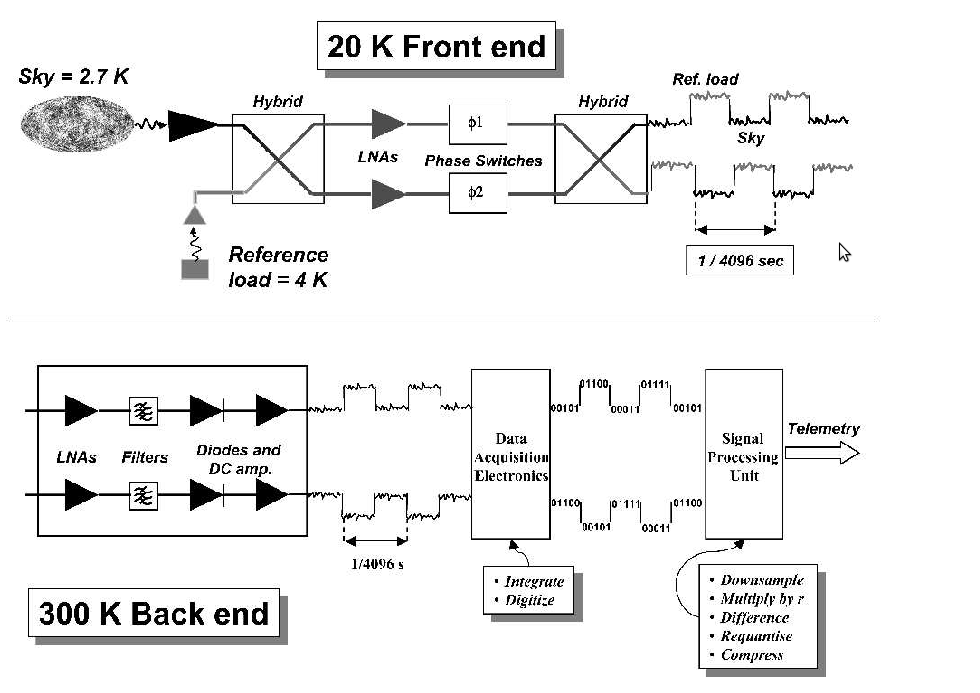
\includegraphics[width=\textwidth]{images/receiver_schematics/pseudo_correlation.png}
 % pseudo_correlation.png: 1920x1200 pixel, 72dpi, 67.73x42.33 cm, bb=
 \caption{The pseudo correlation architecture \protect \cite{Mennella2003b}. The diagram is relevant for one of the orthogonal polarisation states- in the receiver there will be two such signal paths for left and right hand circular polarisation respectively. } 
 \label{fig:pseudo_correlation}
\end{figure}


\begin{sidewaysfigure}
 \centering
 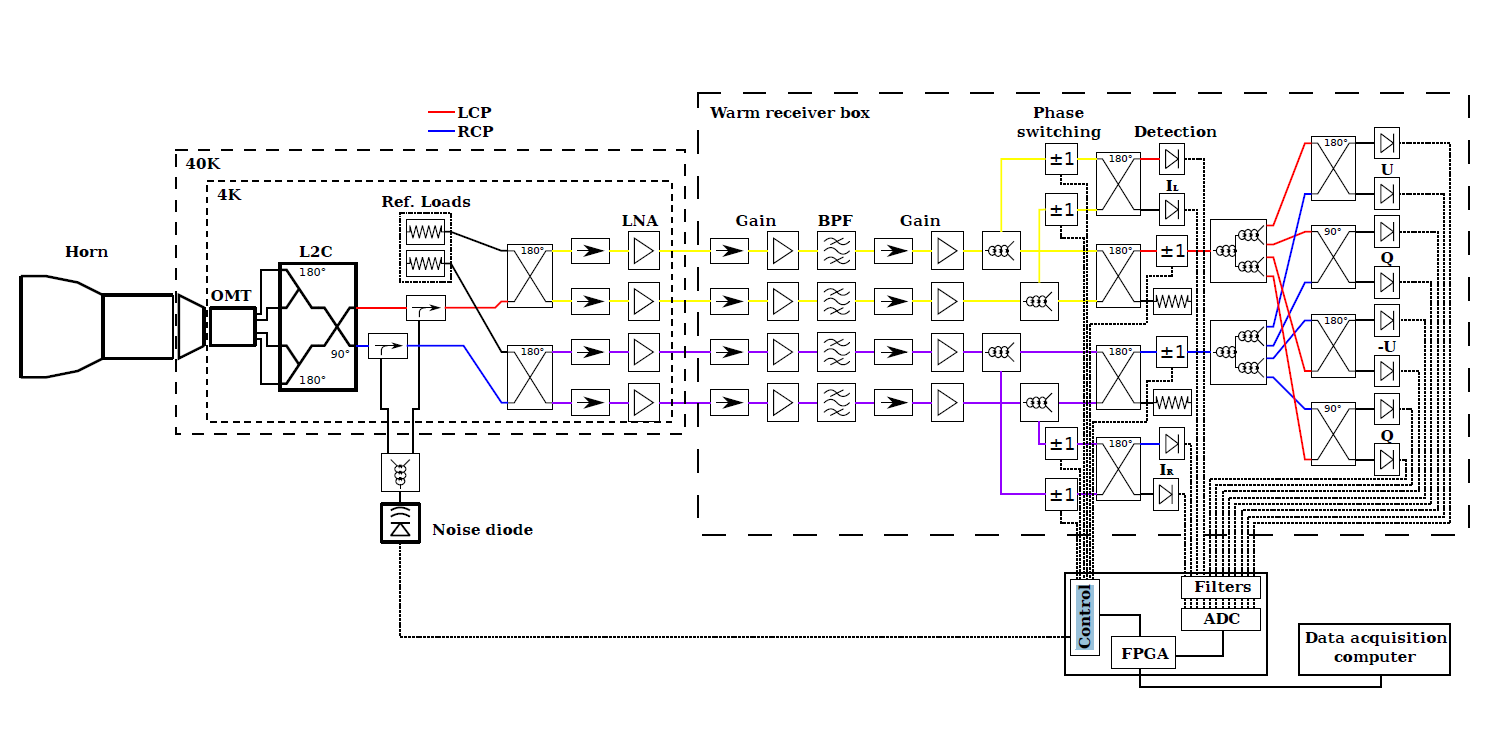
\includegraphics[width=\textwidth]{images/receiver_schematics/analogFull.png}
 % analog.png: 1920x1200 pixel, 72dpi, 67.73x42.33 cm, bb=
 \caption{The pseudo-correlation analog C-BASS radiometer/polarimeter designed by Dr. Oliver King and currently installed on the Owens Valley Antenna \protect \cite{King2009}. The 90\degt phase switch in the front,cold section, converts the linear polarised signal to circular polarised. The signal is then passed through the 180$^{\circ}$ hybrid, coupling in the load signal and amplified. The signal then splits into the radiometer and polarimeter sections. The radiometer signals are phase switched and passed through a second 180$^{\circ}$ hybrid producing a signal similar to that illustrated previously in \fign{fig:pseudo_correlation}. The polarimeter signals are passed through a 180$^{\circ}$ hybrid to remove the load signal, before phase switching and sampling.}
 \label{fig:analog_receiver}
\end{sidewaysfigure}

